% !TEX TS-program = xelatex
% !TEX encoding = UTF-8

% This is a simple template for a XeLaTeX document using the "article" class,
% with the fontspec package to easily select fonts.

\documentclass[11pt]{report} % use larger type; default would be 10pt
\usepackage{fontspec} % Font selection for XeLaTeX; see fontspec.pdf for documentation
\defaultfontfeatures{Mapping=tex-text} % to support TeX conventions like ``---''
\usepackage{xunicode} % Unicode support for LaTeX character names (accents, European chars, etc)
\usepackage{xltxtra} % Extra customizations for XeLaTeX
% \fontspec{"[DroidSerif.ttf]"}
% \setmainfont{Droid Serif} % set the main body font (\textrm), assumes Charis SIL is installed
%\setsansfont{Deja Vu Sans}
%\setmonofont{Deja Vu Mono}
\usepackage[colorlinks,citecolor=red,linkcolor=blue]{hyperref}
\usepackage{amsmath}
\usepackage{xfrac,unicode-math}
\usepackage{siunitx}
\usepackage{mhchem}
\setmathfont[version=cambria]{Cambria Math}
\mathversion{cambria}
\usepackage{cleveref}
% other LaTeX packages.....
\usepackage{geometry} % See geometry.pdf to learn the layout options. There are lots.
\geometry{letterpaper} % or letterpaper (US) or a5paper or....
%\usepackage[parfill]{parskip} % Activate to begin paragraphs with an empty line rather than an indent
\usepackage{placeins}
\usepackage{graphicx} % support the \includegraphics command and options



\newcommand{\lit}{\ce{Li2TiO3}}
\newcommand{\lis}{\ce{Li4SiO4}}
\newcommand{\lio}{\ce{Li2O}}
\newcommand{\liz}{\ce{Li2ZrO3}}
\newcommand{\lial}{\ce{LiAlO2}}
\newcommand{\lisev}{\ce{^7Li}}
\newcommand{\lisix}{\ce{^6Li}}
\sisetup{locale = US}



\title{237D Fusion Technology \\
Introduction to Solid Breeder}
\author{Jon Van Lew}
%\date{} % Activate to display a given date or no date (if empty),
         % otherwise the current date is printed 


\begin{document}
\maketitle
\chapter{Solid Breeder Technology Development}
Lithium appears to be the only material suitable for generating tritium, allowing a self-sustained fuel cycle in a commercial fusion reactor. Aside from liquid lithiums (covered in separate lectures in this course), the most promising lithium materials include solids such as inter-metallic compounds (\textit{e.g.} \ce{Li7Pb2}), lithium oxide (\lio), and ternary oxides (\textit{e.g.} \lis, \lit, \lial, \liz, \textit{etc.}). Solid breeders offer a number of potential safety advantages, including relatively low tritium mobility and low stored chemical energy.

Briefly, lithium-based oxides (including ceramic oxides) are recognized as the best candidate tritium-breeding materials for fusion reactor blankets because several compounds have many desirable characteristics, such as: 
\begin{itemize}
\item{high Li density}
\item{high melting temperature}
\item good tritium release (sufficiently high T release rates and open porosity for purging T)
\item good thermophysical and thermomechanical characteristics
\item ability to withstand the rigors of long-term irradiation at high temperature and under large temperature gradients
\item{desirable neutronics and irradiation characteristics (no bad transmutation nuclides)}
\item{chemical stability \& compatibility with structural material at operating temperatures (in particular thermal stability and chemical inertness are attractive from a safety point of view)}
\end{itemize}

In the following notes, we will go through many requirements of tritium breeding material and details of features that make lithium ceramics attractive. These notes are primarily compiled from many publications on ceramic breeder material development as well as current work on breeder pebble bed modeling. I've attempted to be as succinct as possible to cover the major topics for ceramic breeder materials without sacrificing too many details. But in case of not satisfying this objective, the bibliography at the end of the notes will contain helpful publications that may not be referenced in the text but should be referenced for the curious solid breeder researcher.

A quick note: simulations performed on many candidate materials indicate that inter-metallic compounds have unacceptable operating temperatures (exceedingly narrow temperature windows) and are unattractive for in-situ tritium recovery. In addition, the compounds of \ce{Li7Pb2} and \ce{Li62Pb38} were shown to vigorously react with water and do not offer significant safety advantages compared to liquid breeders. And a major emphasis of blanket/breeder design is placed on safety and environmental acceptability, with primary goals of low tritium inventory in the blanket and minimal long-lived activation products. Therefore in these notes we will not discuss the inter-metallic compounds and focus instead only on candidate materials of lithium ceramics. If you wish to read more on inter-metallics, begin with Clemmer\cite{Clemmer1980} and Abdou \textit{et al.}



\section{Material Requirements}
For each candidate breeder, a number of performance criteria were established in design studies in the late 1970s and early 1980s. The outcome of the studies are summarized in the following list of material property requirements:
\begin{enumerate}
\item Neutronics
\item Thermochemical Properties
\item Tritium Release
\item Physical/Thermo-physical Properties
\item Compatibility
\item Radiation Effects
\item Fabrication
\end{enumerate}

We will go through the different material requirements and introduce the analysis involved with evaluating material for each requirement. In the time since the solid breeder concept was introduced, a rich experimental database has begun to develop for a number of candidate ceramic materials. The introduction given in these notes will not be comprehensive but should provide a starting point for understanding the physics behind the material requirements.

\subsection{Neutronics of lithium}
Natural lithium occurs with the isotopic abundances of 92.58\% for \lisev~and 7.42\% for \lisix~. At low neutron energies, the major tritium and heat producing neutron reaction in lithium ceramics is associated with the \lisix~isotope:
\begin{align}
\ce{n + ^6Li -> He + T} + \SI{4.78}{\mega\electronvolt} \label{eq:Li6T}
\end{align}
The cross-section for this reaction is given in \Cref{fig:xsects}. \lisix~has a very high neutron capture cross-section (3,000 barns) for thermal neutrons $E \approx 10^{-1}$ to $10^{-2}$ eV. Yet, at high neutron energies (\SI{14}{\mega\electronvolt}), such as those found near the first wall of a fusion reactor, the neutron cross section of \lisix~drops to less than 0.1 barn, effectively precluding the \lisix~reaction with virgin fusion neutrons. In reality, the high energy neutrons are slowed from collisions with the structural material in the first wall and blanket. Consequently, \lisix~reaction rates near the first wall are highly dependent on the ability of first walls and blankets to moderate neutron energies.

\begin{figure}[ht]
\centering
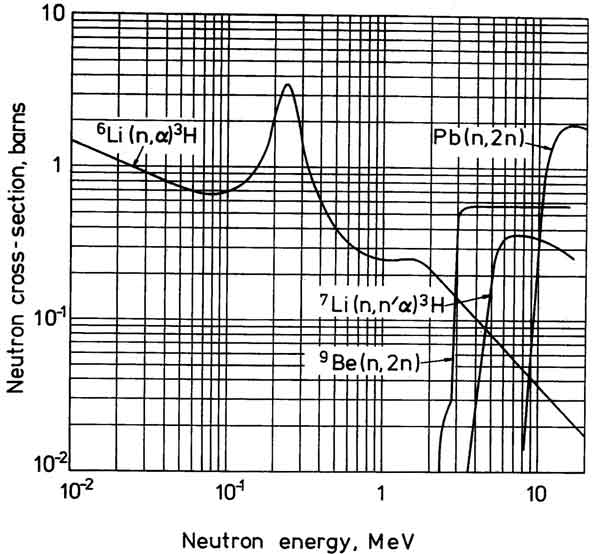
\includegraphics[width=0.8\textwidth]{../images/breeding_xsecs} 
\caption{Cross-sections of various blanket materials. Note the threshold for the \lisev~and neutron multiplying reactions.}
\label{fig:xsects}
\end{figure}

Neutron multipliers such as lead and beryllium not only moderate \SI{14}{\mega\electronvolt} neutrons, yielding a softer neutron spectrum for increased \lisix~reactions, but also generate additional neutrons from (n,2n) reactions. Neutron multiplication materials will be discussed again shortly.

\lisev~interactions with neutrons, being endothermic, possesses a threshold energy below which it will not react with neutrons. It does, however, have a small but significant cross-section (around 1 barn) for neutrons with energies greater than 5 MeV. The \lisev~reaction is:
\begin{align}
\ce{n + ^7Li -> n + He + T}-\SI{2.47}{\mega\electronvolt}\label{eq:Li7T}
\end{align}
where the reaction releases a lower energy neutron which is immediately available for capture by \lisix~atoms. Due to \lisev~ability to act as neutron multiplier, \lio, with a high lithium atom density, is potentially capable of attaining adequate tritium breeding ratios without an external neutron multiplication material. Several atomic densities of lithium for select candidate materials are given in \Cref{fig:li-density}. Aside from \lio~, all ternary oxides require neutron multiplication due to lower lithium density.

\begin{figure}[ht]
\centering
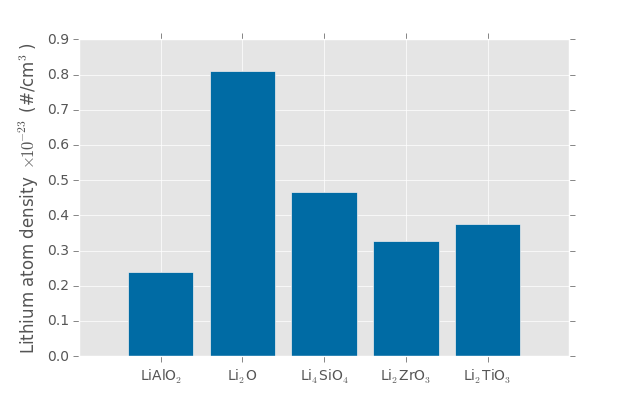
\includegraphics[width=0.8\textwidth]{images/li-density} 
\caption{Lithium oxide is the only ceramic with lithium density sufficiently high to potentially operate without a neutron multiplier. All other ternary oxides have comparable lithium densities.}
\label{fig:li-density}
\end{figure}
 %However, as will be shown next, \lio~has very high tritium solubility to the extent that tritium inventories in \lio~may be unacceptably high.

 %Lithium metal is soft, has a low density (of 0.53 g/cm$^3$), and has a physical appearance similar to lead. 

% Mean-free-path of tritium-producing reaction in natural lithium
% \begin{align*}
% \lambda_t & > \SI{70}{\centi\meter} && n(\SI{14}{\mega\electronvolt})\\
% \lambda_t & \approx \SI{2}{\centi\meter} && n(\SI{1}{\electronvolt}) 
% \end{align*}

% In 90\% enriched \lisix~,
% \begin{align*}
% \lambda_t & \approx \SI{0.15}{\centi\meter} && n(\SI{1}{\electronvolt}) 
% \end{align*}
% \lisix~cross-section at \SI{0.025}{\electronvolt} is %\SI{740}{\barns}.



\subsection{Thermochemical Properties}
Vapor pressure, phase equilibria, thermal stability, and thermodynamics are several of the thermochemical properties important to the study of ceramic breeder materials. 
% Li2O, only ceramic that could possible achieve TBR>1 without dedicated neutron multiplier. Highly hygroscopic.
% Li2O + H2O -> 2LiOH deltaH = 128.9 kJ/mol
% LiOH is highly corrosive

A major concern of candidate materials is the solubility of tritium in the material; too high of solubility will lead to unacceptable levels of tritium inventory. A simplified calculation can be performed on the lithium oxides to predict the function of \ce{T2O} partial pressure in gas phase. Assuming: 1) thermochemical data of hydrogen applies to tritium; 2) isotope effects are not considered; 3) tritium exists in the form of \ce{LiOT} in solid solution; and 4) activity coefficients of all species are unity. We can then calculate the partial pressure of oxides as:
\begin{align}\label{eq:liot-equilibrium}
\ce{2LiOT + MO_X <=> Li2MO_{X+1}}
\end{align}
and
\begin{align}
p(T_2O) = X_MX^2K_p
\end{align}
where $p(T_2O)$ is the partial pressure of \ce{T2O}, $X$ is the mole fraction of LiOT, and $X_M$ is the mole fraction of the binary metal oxide (\textit{e.g.} \ce{TiO3}). 

As neutrons transmute lithium from the ceramic, the stoichiometry of the material will begin to change. There is great uncertainty in the activity of lithium-depleted species. The lithium depleted species may not exist in the simple metal oxide form (\textit{e.g.} \ce{Al2O3}) but most probably another ternary compound (\textit{e.g.} \ce{LiAl5O8}). In the examples of lithium aluminate, \ce{LiAl5O8} is more stable than \ce{LiAl2O3} and therefore free energy changes and $k_p$ values for reactions may be overestimated. Moreover, the composition of the breeding material continuously changes during operation of the blanket because of lithium burn-up. Because tritium is being removed from the blanket, the mole fraction of \ce{LiOT} will reach a constant value. However, the concentration of other specie (metal oxides) will continuously increase.

Although there is considerable uncertainty in many of the terms of \Cref{eq:liot-equilibrium}, approximations can be made for many of the candidate ceramics. Equlibrium tritium concentrations in solid ceramic breeders for a \ce{T2O} partial pressure of \SI{1.3}{\pascal} were calculated by Clemmer and his results are reproduced in \Cref{fig:solubility}.\cite{Clemmer1980}

\begin{figure}[ht]
	\centering
	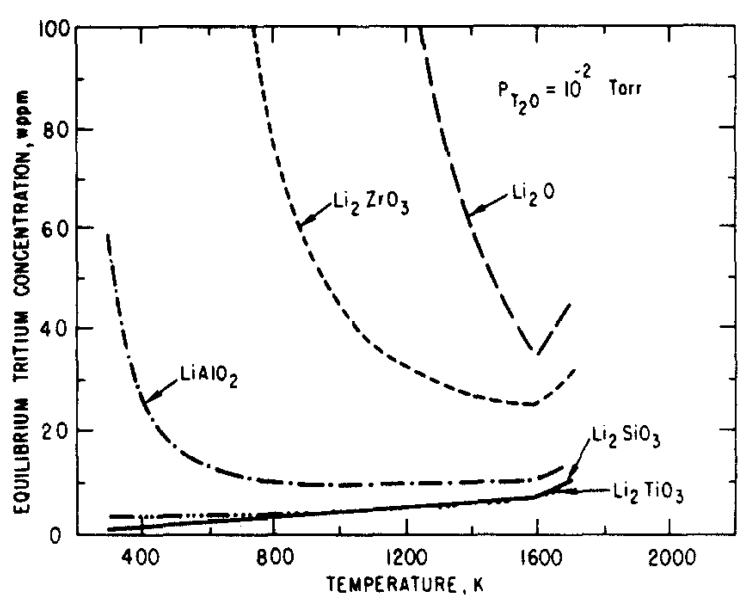
\includegraphics[width=0.75\textwidth]{images/solubility} 
	\caption{Calculated equilibrium tritium concentrations in candidate solid breeding materials at $P_{T_2O} = \SI{1.3}{\pascal}$.}
	\label{fig:solubility}
\end{figure}

From estimates of solubility shown in \Cref{fig:solubility}, it is immediately apparent that all the ternary oxides have significantly lower tritium ``solubilities'' than \lio. In spite of the promising feature of \lio~being capable of existing without a neutron multiplier due to its high lithium density, the tritium inventory of the material may be unacceptably high.

% Lastly, because safety as a key issue supporting fusion reactors, we must consider that lithium is chemically reactive with oxygen. Two interactions are:
% \begin{align*}
% 2\mathrm{Li} + \frac{1}{2}\mathrm{O} &\rightarrow \mathrm{Li}_2\mathrm{O} - 142.75~\text{kCal/mol}\\
% 2\mathrm{Li} + \mathrm{O} &\rightarrow \mathrm{Li}_2\mathrm{O}_2 - 151.9~\text{kCal/mol}
% \end{align*}
% Lithium will exothermically react with water (or air, concrete, or any moisture-containing materials) with high amounts of energy released. Of primary concern in lithium fires is the peak flame temperature. This will determine, to a large extent, whether many radioactive species become air-borne by vaporization. The flame temperature depends on many variables. Some investigations found it to be about \SI{2500}{\kelvin} which would cause some materials to melt but not vaporize.

%Vaporization data for several candidate ceramics is discussed by Johnson \textit{et al.}.\cite{Clemmer1980}; showing that higher lithium vapor pressures exist for materials with higher lithium content.

\subsection{Tritium Release and Recovery}
Tritium recovery from solid tritium-breeding materials is a key factor in establishing the viability of the solid-breeder concept. Designs of solid breeders have tritium removed with a purge gas (primarily helium) flowing through the open porosity of packed beds of lithium ceramics. The feasibility of the solid breeder concept is based on the capability of tritium to readily transport from the solid ceramic into the purge gas. Tritium release is a function of grain size, microsctructure, and open/closed porosity. To understand the capability of tritium removal, five mechanistic steps are identified for bred tritium to be recovered (visualized in \Cref{fig:mechanisms_tritium_transport}) . The steps follow as
\begin{enumerate}
\item bulk diffusion,
\item desorption of tritium (T$_2$O),
\item grain boundary migration,
\item percolation of tritium through pores internal to the solid ceramic toward the flowing purge gas,
\item convective mass transfer out of the blanket via purge channels.
\end{enumerate}

\begin{figure}[ht]
	\centering
	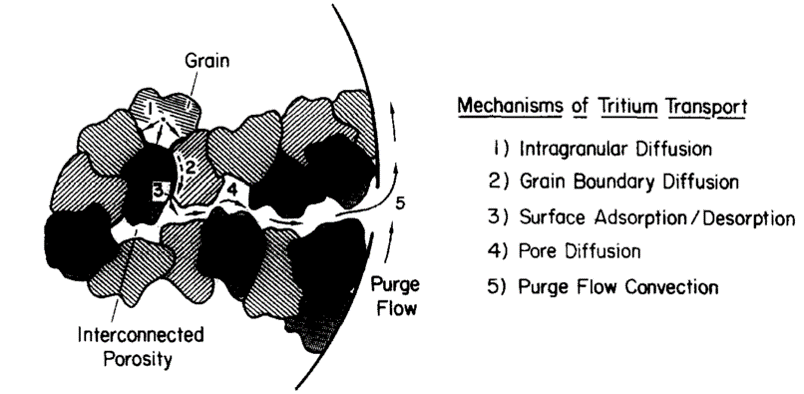
\includegraphics[width=0.75\textwidth]{images/mechanisms_tritium_transport} 
	\caption{Mechanistic steps of tritium transport through ceramic materials into the purge gas for removal.}
	\label{fig:mechanisms_tritium_transport}
\end{figure}

Bulk diffusion of tritium is considered to be a significant contributor to tritium inventory. For spherical particles of radius $r$, assuming zero surface concentration, the tritium inventory $T$ is given by 
\begin{equation}\label{eq:inventory-diff}
T = \frac{1}{15}\dot{T}\frac{r^2}{D}
\end{equation}
where $\dot{T}$ is the tritium generation rate and $D$ is diffusivity of tritium in the ceramic. It is significant to note that the tritium inventory is a function of the square of the particle size. Thus it is clear that small grain sizes are required for minimum tritium inventory and that the grains should not significantly grow during the lifetime of a reactor blanket. Diffusivity values of tritium in ceramics are extremely scarce and with much uncertainty. Kinetic experiments of post-irradiation tritium release from several candidate breeders have been performed. The kinetics in the experiments are non-steady-state and the diffusivity is given by 
\begin{equation}\label{eq:exp-diff}
D = 0.16 \frac{r^2}{\tau}
\end{equation}
where $\tau$ is the mean residence time, defined as the time required to extract 87.4\% of the tritium. Combining \Cref{eq:inventory-diff} and \Cref{eq:exp-diff} eliminates diffusivity and radius (with large variation between particles and grains), yielding:
\begin{equation}
T = 0.42 \dot{T}\tau
\end{equation}

We can then estimate the diffusive inventory in a blanket based on the readily-measured residence time, $\tau$. It must be kept in mind that the particular micro-structure of the ceramics measured in kinetic experiments must correspond to the micro-structure of the material in the blanket in order for the diffusivity predictions to hold.

The tritium generation rate, $\dot{T}$ is a function of the fusion reactor power output and blanket design. Assuming this value is known for a given blanket, residence times have been measured to be temperature dependent which is consistent with diffusion-controlled processes. Therefore, based on the present model, the range of operating limitations are defined on the low end where bulk diffusion is the rate-limiting step. A minimum temperature is defined as the temperature at which the tritium inventory exceeds \SI{1}{\kilo\gram\per\giga\watt}. The minimum temperatures for many candidate materials are shown (from various sources) in \Cref{fig:Tmin}. Minimum temperatures generally range from 300 up to \SI{500}{\celsius}.

\begin{figure}[ht]
	\centering
	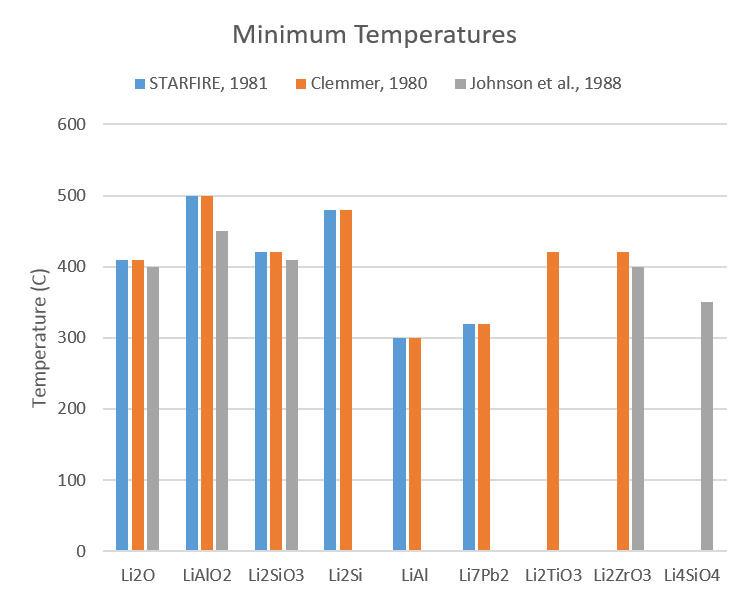
\includegraphics[width=\textwidth]{images/Tmin} 
	\caption{Minimum temperatures for various candidate materials (compiled from various sources) based on rate-limiting diffusion processes.}
	\label{fig:Tmin}
\end{figure}

The other end of the operating limit is based on restructuring or grain growth in ceramics which can greatly affect the diffusive inventories; calculated inventories vary as the square of the grain size and should be kept small. When ceramic materials are heated above their sintering temperature, generally in excess of $0.8 T_\text{melt}$ (in absolute temperature), grains will grow. The effects of sintering at \SI{1200}{\celsius} over a number of hours is shown in \Cref{fig:material-production-NFRI} (images courtesy of Yi-Hyun Park from NFRI). Grain growth, as witnessed in these images, must be avoided in operation.

\begin{figure}[ht]
	\centering
	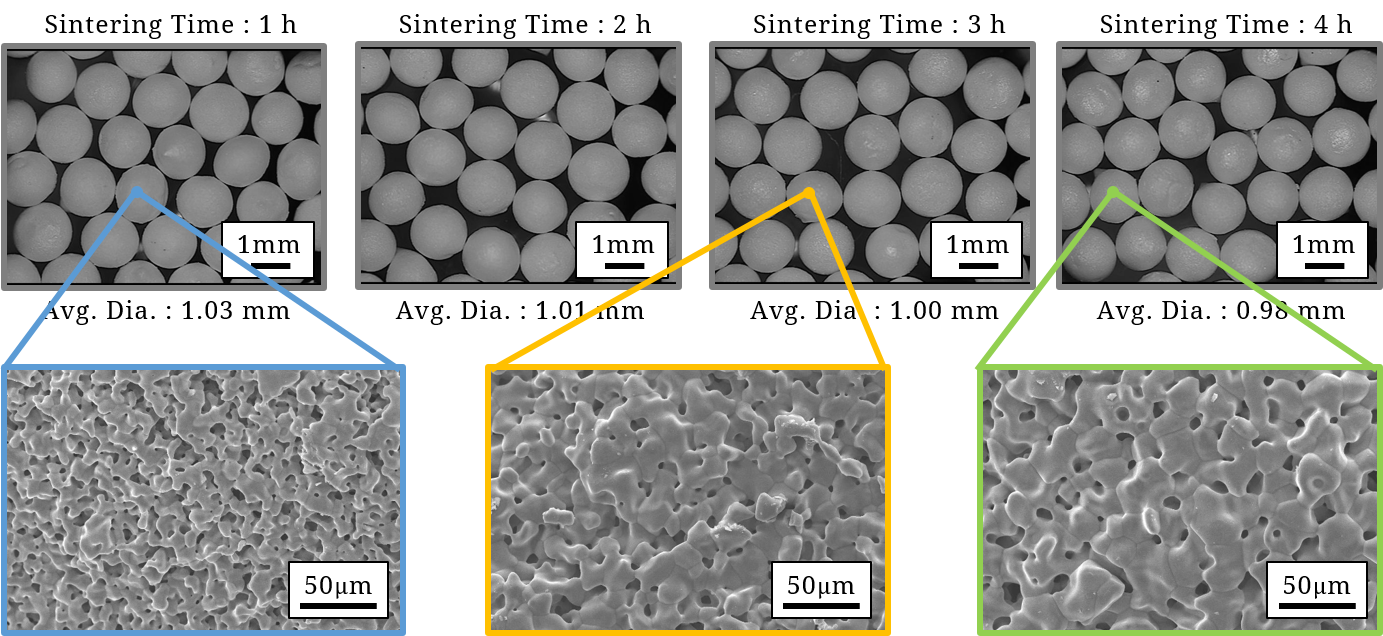
\includegraphics[width=\textwidth]{images/material-production-NFRI} 
	\caption{Maximum temperatures for various candidate materials (compiled from various sources) based on irradiated sintering temperatures ($0.6T_\text{melt}$).}
	\label{fig:material-production-NFRI}
\end{figure}

Moreover, neutron radiation typically enhances sintering characteristics and lowers the sintering temperature; the effects of radiation are expected to reduce the sintering temperature to $0.6 T_\text{melt}$.\cite{Johnson1981} Maximum temperatures are thus set by sintering, the candidate materials are compared in \Cref{fig:Tmax}

\begin{figure}[ht]
	\centering
	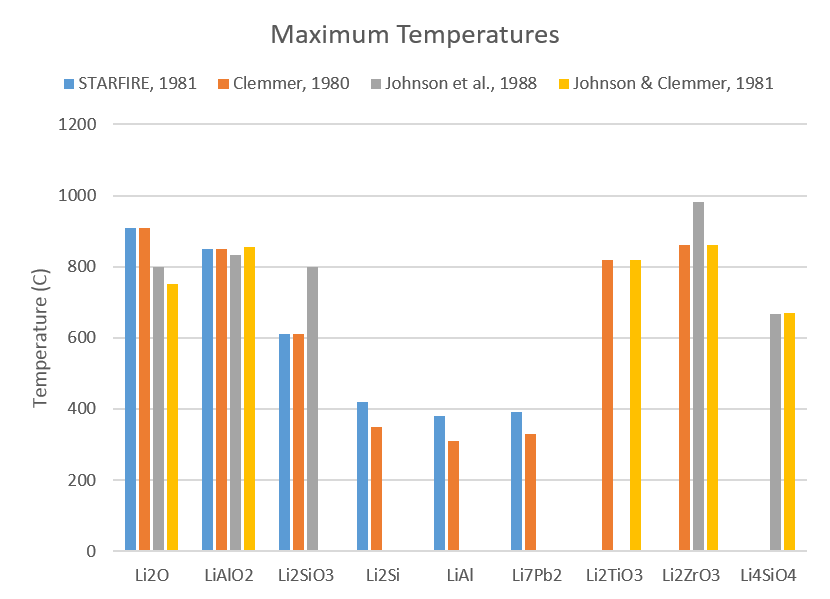
\includegraphics[width=\textwidth]{images/Tmax} 
	\caption{Maximum temperatures for various candidate materials (compiled from various sources) based on irradiated sintering temperatures ($0.6T_\text{melt}$).}
	\label{fig:Tmax}
\end{figure}

In general, acceptable candidate materials have their maximum temperature between 750 and \SI{900}{\celsius}. 

As a consequence of the tritium release from the solid breeder material, we are faced with a relatively narrow operational temperature to which solid breeder designers must adhere. Thus to provide designers the ability to optimize breeder volumes for tritium breeding and subsequent tritium release, we must understand the important physics and phenomena dictating thermophysical properties and thermomechanical responses of pebble beds during operation in a fusion reactor.


\FloatBarrier
\subsection{Physical \& Thermophysical Properties}
The temperature window established for tritium release dictates the thermal characteristics of pebble beds become critically important to understand. Candidate ceramic materials is itself quite low, being reduced by porosity. Several candidate conductivities are given in \Cref{fig:k_s} assuming 80\% theoretical density; \lit~has comparable conductivities with \lis.

\begin{figure}[ht]
	\centering
	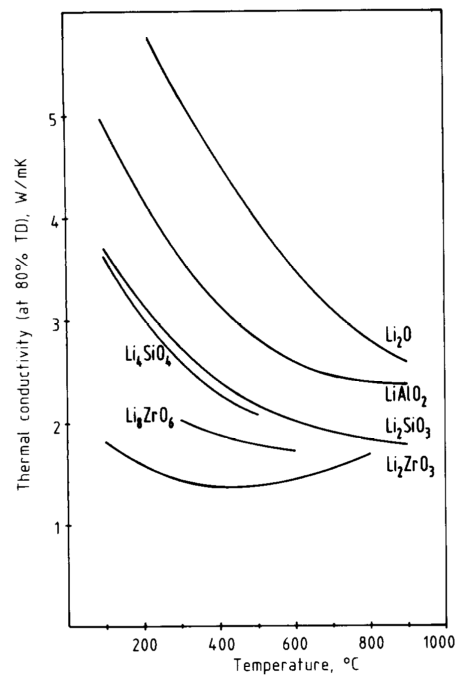
\includegraphics[width=0.45\textwidth]{images/k_s} 
	\caption{.}
	\label{fig:k_s}
\end{figure}

In sphere-pac form, the effective conductivity drops well below the solid conductivity. Measurements of effective thermal conductivity for \lis~and \lit~are given in \Cref{fig:k_eff} for different interstitial gases and packed bed temperatures. In a stagnant helium environment, the effective conductivity values for both materials fall to around \SI{1}{\watt\per\meter\per\kelvin}.
\begin{figure}[ht]
	\centering
	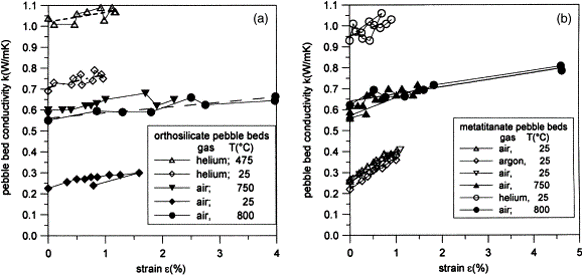
\includegraphics[width=\textwidth]{images/k_eff} 
	\caption{.}
	\label{fig:k_eff}
\end{figure}



The material integrity is a function of pebble size distribution, sphericity, mechanical strength, chemical stability.
% \lit~has acceptable Li density, not hygroscopic, has lower activation, similar T release to \liz. Mechanically stronger than \lis.
% \lis~has weak crush strength, acceptable Li density, stable (can't read my notes)

\FloatBarrier 
\subsection{Compatibility}
Compatibility studies have been carried out at several temperatures between various couples of breeder materials and structural materials.\cite{Johnson1988} \ce{Li5FeO4}, \ce{Li2CrO2}, and \ce{Li2Ni8O10} were common corrosion products (varying by structural material). \lio~was seen to be most reactive; reaction rates for \lis, \liz, and \lial~were much lower. However, in studies of \lio~where the material was rigorously freed of moisture impurity, \lio~was found to be inert to metals. Corrosion properties of \lio~are therefore attributed to the presence of highly corrosive LiOH contamination happening in the presence of water with \lio. In general, reaction rates increase with increasing temperature and moisture content.\cite{Johnson1991}

Interaction of ternary oxide ceramics with beryllium was found to be counter to expectations based on thermodynamics and seen to be negligible up to \SI{650}{\celsius} for \lis, up to \SI{700}{\celsius} for \lial~and \liz, for durations up to 3000 hours. A beryllium oxide layer is assumed to form on the material surface, thereby protecting it from further oxidation. The SIBELIUS experiment studied the effect of neutron irradiation on the \ce{BeO} layer. Data from SIBELIUS indicate the beryllium oxide layer appears to have some influence on the amount of tritium retained by the beryllium discs. The tritium release from the ceramics, on the other hand, is consistent with other tritium release measurements of the ceramic materials in the absence of beryllium and therefore appears to not be affected by adjacent beryllium.\cite{Kopasz1995,Roux1992}

\subsection{Radiation Effects}
We have already discussed the anticipated effect of radiation on lowering predicted sintering temperatures of candidate ceramic materials. While in a fusion reactor, the ceramic materials will subjected to high temperatures and changing material characteristics from the neutron environment. The neutron capture reaction of \ce{n + ^6Li -> T + He} produces significant lattice damage during irradiation.\cite{Johnson1981} Not only are two large gas atoms produced, one of which is not expected to be soluble in the parent material, but also a lithium vacancy is produced. Several anticipated radiation damage mechanisms are:
\begin{itemize}
\item Displacement Damage
	\begin{itemize}
	\item Vacancies
	\item Loops, Clusters, etc.
	\item Interstitials
	\end{itemize}
\item Reaction Products
	\begin{itemize}
	\item Bubbles
	\item Interstitials
	\item Substitutional Defects
	\end{itemize}
\item Lithium Depletion
	\begin{itemize}
	\item Vacancies
	\item Oxygen Excess
	\item Nonstoichiometry
	\end{itemize}
\item Microstructural
	\begin{itemize}
	\item Sintering
	\item Grain Growth
	\item Microcracking
	\end{itemize}
\end{itemize}
and the manifestation of these atomistic changes as microstructural damage must be evaluated with irradiation experiments.

In lithium ceramics there are a minimum of two sublattices composed of anions and cations. Creation of more defects on one sublattice than the other, for instance on the oxygen lattice, would lead to charge separation within the matrix. If sufficient defect mobility exists, the newly formed defects can annihilate or cluster, forming voids or precipitates within the crystal. Displacement damage to lattices is quantified with a value displacements per atom, dpa. In fusion reactors, solid breeder materials will receive substantial displacement damage from high energy neutrons of the plasma. Fusion neutrons that have been slowed (from interaction with neutron multiplication or structural materials) to lower energies will produce much less displacement damage.

Helium generated in the solid breeder material during irradiation, owing to its inert nature, will have a much lower solubility in ceramics than tritium, since only interstitial positions are available. The lower solubility for helium will result in a lower permeability so that the rate of migration out of the lattice will be less. Moreover, low solubility will enhance bubble formation and swelling.

A consequence of neutron capture is loss of lithium atoms from ceramic lattices. This loss creates either a lithium vacancy or a localized excess of oxygen, \textit{i.e.} oxygen interstitials. Since tritium ions are created during the neutron capture of a lithium ion, the overall electrostatic equilibrium of the crystal is maintained. When the tritium ions are subsequently released to the purge gas, it necessarily follows that the oxygen ions must also be released in order to avoid a charge buildup in a single valency system. If multivalent ions (\textit{e.g.} \ce{Fe^{+2}}, \ce{Fe^{+3}}) are present, then a change in oxidation states would balance the charge of the excess oxygen. From this point of view, it is natural that we observe tritium released as \ce{T2O} in \lio~systems rather than as a hydrocarbon or \ce{T2}.\cite{Johnson1981}

Lastly, as discussed in the discussion of thermochemistry of candidate ceramics, as lithium depletion (or lithium burn-up) occurs to a significant extent (around 5\%), the resultant nontsoichiometry in ternary oxides could establish rather than single-phase condition. For example, under irradiation and lithium burn-up, \lis~would lead to an excess of silica and the melting point of the \SI{1300}{\celsius} to a eutectic temperature of \SI{1024}{\celsius}. Such a reduction in melt temperature would have significant impact on sintering and tritium inventory in the solid breeders.\cite{Johnson1981}

Irradiation experiments are ongoing 
\cite{vanderLaan200099}

\section{Neutron Multiplication in Solid Breeders}
\begin{align}
\ce{n + ^9_4Be -> 2n + 2He + T}-\SI{1.57}{\mega\electronvolt}\label{eq:Be-n}
\end{align}

melting temperature of beryllium is \SI{1250}{\celsius}, melting temperature of lead is \SI{327}{\celsius}. Thermal energy of \ce{Be} is \SI{1.7}{\mega\electronvolt}, \ce{Pb} is \SI{7}{\mega\electronvolt}. Choose beryllium for non-mobile breeder.

Chemical composition of beryllium,
\begin{itemize}
\item{BeO}
\begin{itemize}
\item{excellent compatibility with structural steel}
\item{carcinogen, causes beryllium disease if inhaled}
\end{itemize}
\item{Be}
\begin{itemize}
\item{incompatibility with structure steel, forming \ce{FeBe13}}
\item{\ce{Be} reaction with water forming \ce{BeO} (\ce{Be + H2O -> BeO + H2})}
\item{\ce{2Be + O2 -> 2BeO}}
\end{itemize}
\item{Be12Ti}
\begin{itemize}
\item{compatible with ss.}
\item{high melting temperature}
\item{less swelling than Be}
\item{higher chemical stability}
\item{high Be density maintains neutron multiplication characteristics}
\end{itemize}
\end{itemize}
Bear in mind limited Be abundance on Earth. (remember Homework set)

Beryllium will also exist as a pebble bed. The following reaction has small probability of occurrence (check cross-section for this reaction)
\begin{align*}
\ce{n + ^9_4Be -> ^4He + ^6He} \\
\ce{^6He -> ^6Li + beta^-} \\
\ce{n + ^6Li -> He + T}
\end{align*}

Diffusional release of T from irradiated beryllium is very slow, measured in \ce{BeO} to be about \num{1e-15} cm2/sec at \SI{900}{\celsius}. The diffusional path should be kept around 1 micron for T inventory concerns.




\subsection{Fabrication}
One last point to discuss on ceramic materials before moving on to a discussion of neutron multipliers concerns fabrication. Candidate ceramic material feasibility is in part dependent on the fabrication price and ability to scale to industrial output quantities. While this is an important point for realiziation of solid breeders, it will not be discussed in detail here. van der Laan \textit{et al.}\cite{vanderLaan200099} and Johnson \textit{et al.}\cite{Johnson1991} provide thorough descriptions and discussions for various fabrication techniques.



































\chapter{Introduction to Solid Breeder Designs}
The solid breeder concept with sphere-pac beds satisfies the requirements of a breeder unit: transmute lithium into tritium, act as shield to other sensitive equipment and personnel, and convert energy into extractable heat for electricity production. Common features of pebble bed designs are:
\begin{enumerate}
\item{Always separately cooled with (with \textit{e.g.} helium or water)}
\item{Necessity of neutron multiplication}
\item{Surrounded by a structure of reduced-activation ferritic steel}
\end{enumerate}
In a typical solid breeder module, the module is subdivided into several alternating layers of neutron multiplication material (generally beryllium) and tritium breeding material. The layers are separated by steel plates with internal channels for coolant. A conceptual design of the Japanese solid breeder for ITER is shown in \Cref{fig:japanese-breeder-design}.

\begin{figure}[ht]
	\centering
	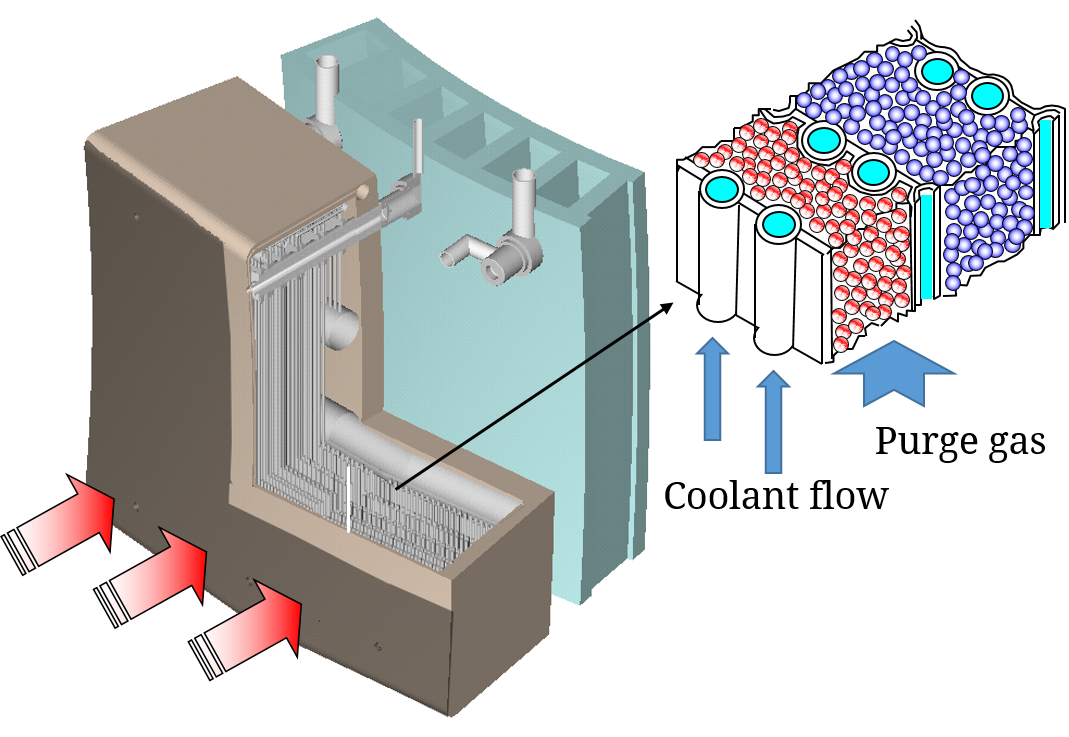
\includegraphics[width=0.6\textwidth]{images/japanese-breeder-design} 
	\caption{Sketch of a typical unit of a pebble bed tritium breeding zone. The pebble bed is cooled with contact to the containing structure.}
	\label{fig:japanese-breeder-design}
\end{figure}

All heat deposited into the ceramic pebble beds is conducted towards the structure and into coolant. Coolant proceeds out of the tritium breeding module and into a standard electricity production cycle where heat is extracted. After tritium is generated inside the ceramic, the bred tritium is ultimately carried away by a low-pressure, slow moving purge gas (primarily helium) and extracted in a closed loop for fuel. Pebble bed forms of tritium breeding volumes have several advantages which include: large surface area to volume, ease of assembly of granular materials into complex geometries, bred tritium can be readily removed with large open porosity between pebbles, and temperature gradients across any single pebble are small enough to avoid damage from thermal stress. A sketch of a generic volume of ceramic pebble bed is given in \Cref{fig:solid-breeder-sketch}

\begin{figure}[ht]
	\centering
	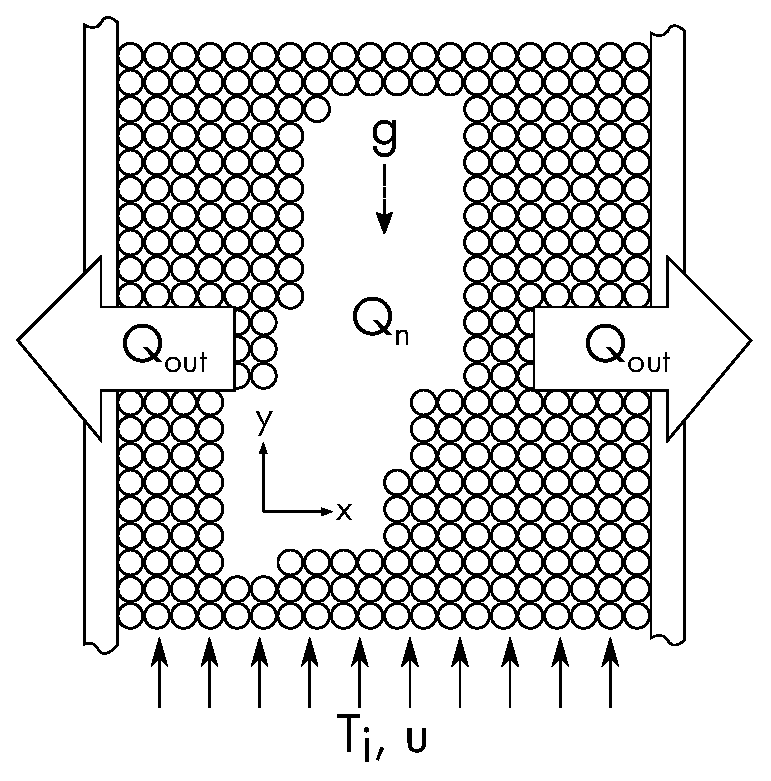
\includegraphics[width=0.6\textwidth]{images/x-domain} 
	\caption{Sketch of a typical unit of a pebble bed tritium breeding zone. The pebble bed is cooled with contact to the containing structure.}
	\label{fig:solid-breeder-sketch}
\end{figure}

\section{Purge gas}
Purge - keep delta-P around 0.01 MPa. mdot = 0.1 to 0.3 g/s.

Pressure drop (per unit length) for the purge gas can be calculated based on the Kozeny-Carman correlation; derived for packed beds at the close-packed limit,
\begin{equation}\label{eq:K-C-pressure}
    \frac{\Delta p}{L} = \frac{180 \bar{U} \mu}{d_p^2} \frac{(1-\epsilon)^2}{\epsilon^3}
\end{equation}
where $\mu$ is the viscosity, $\epsilon$ is the void fraction, $d_p$ is the particle diameter (assuming spherical) and $\bar{U}$ is the superficial velocity of the fluid in the packed bed.

Carman points out the limitations of applicability of the Kozeny-Carman (KC) equation: built into the equation is the assumption that the range of pore size and shape is fairly isotropic and similarly the tortuosity through the packed bed is relatively uniform. Pressure drop as a function of Reynolds number for \SI{1}{\milli\meter} particles in a packing fraction of $\phi = 1-\epsilon = 0.645$ in helium at \SI{600}{\celsius} is given in \Cref{fig:KC-pressure-drop}.

\begin{figure}[ht]
    \centering
    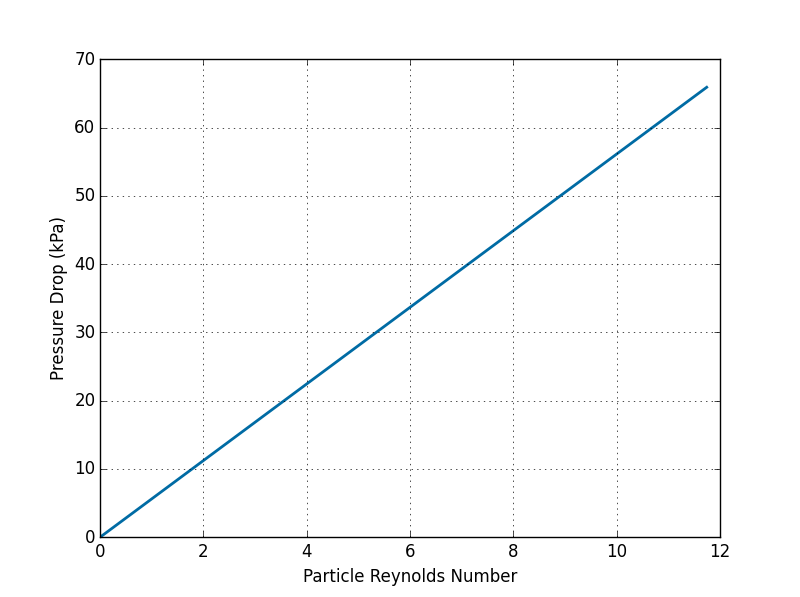
\includegraphics[width=0.75\textwidth]{images/KC-pressure-drop}
    \caption{Kozen-Carman pressure drop increases linearly with particle Reynolds number.}
    \label{fig:KC-pressure-drop}
\end{figure}

\section{Coolant}

Example values: coolant - P = 8 MPa. Tin = 300 C, Tout = 500 C (kept below 600 C for structural integrity of container).

Nothing exotic. standard heat transfer of a fluid in a duct. Must consider safety issues of high pressure coolant.

\section{Effective Conductivity of Packed Beds}
One approach to studying heat transfer granular material is to treat the packed bed as a fictitious continuous media. Many experiments have been carried out for developing phenomenological models of effective material properties. In this approach, heat transport in pebble beds is often characterized with an effective thermal conductivity, $k_\text{eff}$, and interface heat conductance. Many models have shown their ability to accurately predict the temperature profiles for pebble beds under specific operating conditions. We begin with a review of $k_\text{eff}$ correlations.

Deissler and Boegli, in 1958, proposed upper and lower bounds of effective thermal conductivity, $k_\text{eff}$, in two-phase granular media to be given by alternating layers of the two phases arranged in parallel or series, respectively \cite{Deissler1958}. In the case of parallel layers, effective conductivity, normalized by fluid conductivity, is
\begin{equation}\label{eq:keff-parallel}
	\frac{k_e}{k_f} = \epsilon + (1-\epsilon)\kappa
\end{equation}
where $k_f$ is the fluid conductivity, $\kappa = k_s/k_f$ is the ratio of solid to fluid conductivity, and $\epsilon$ is the void fraction in the porous media. Similarly, the minimum effective conductivity is found in a serial layering of the solid and fluid phases,
\begin{equation}\label{eq:keff-series}
	\frac{k_e}{k_f} = \frac{1}{\epsilon + (1-\epsilon)/\kappa}
\end{equation}
\Cref{eq:keff-parallel,eq:keff-series} act as theoretical upper and lower limits to true effective thermal conductivities of real material.

One of the most widely-used correlations was put forth by Zehner and Schlunder in 1970 \cite{Zehner1970,Zehner1972}. They considered a cylindrically-shaped unit cell and made the analogy between heat and mass transfer to derive an empirical fit to data in the bulk of two-phase porous media. The Zehner-Schlunder (ZS) correlation is
\begin{equation}
    \frac{k_e}{k_f} = \left(1-\sqrt{1-\epsilon}\right)+\frac{2\sqrt{1-\epsilon}}{1-B/\kappa}\left[\frac{(1-1/\kappa)B}{(1-B/\kappa)^2}\ln\left( \frac{\kappa}{B} \right) - \frac{B+1}{2} - \frac{B-1}{1-B/\kappa}\right]
\end{equation}
where $B$ is a deformation parameter related to porosity as
\begin{equation}\label{eq:zs-B}
    B = 1.25\left(\frac{1-\epsilon}{\epsilon}\right)^{1.11}
\end{equation}

Over the years, many other correlations have been developed for predicting effective conductivity of packed beds. Some focus on conditions of higher porosity, consider radiation effects, or situations of large $\kappa$. A number of correlations have been plotted together along with the three presented here; given in \Cref{fig:kappa-experimental-comet}. Plotted on the figure is also a compilation of experimental data from many sources (reproduced from Ref.\cite{VanAntwerpen2010}) and recent COMET data recorded for graphite material at UCLA.

\begin{figure}[ht]
    \centering
    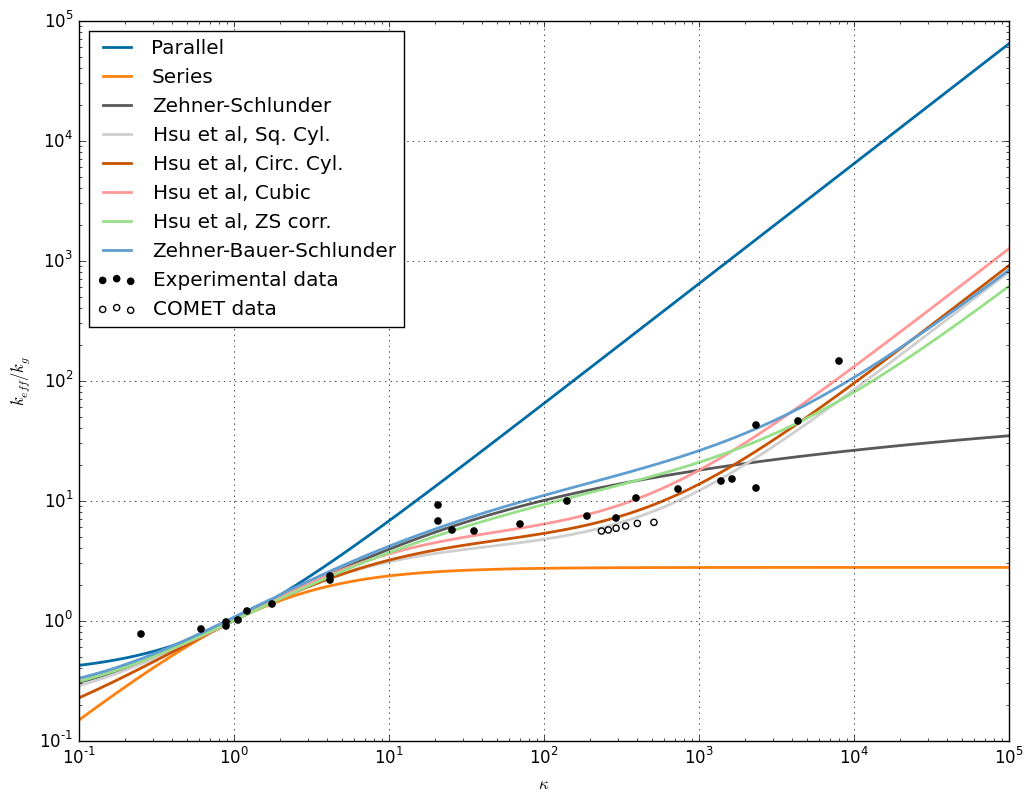
\includegraphics[width=\textwidth]{images/keff-kappa-experimental-comet}
    \caption{Comparison of COMET data on IG11 graphite, $k_\text{eff}$ correlations, and experimental data. Data compiled by \cite{VanAntwerpen2010} from many sources and measured data at UCLA.}
    \label{fig:kappa-experimental-comet}
\end{figure}


However, the accuracy of the model predictions often degrade as soon as a pebble bed's granular material, grain radii distributions, or operating conditions vary from the experimentally studied packed beds. In addition, propensity for creep, crushing, and inter-particle sintering of ceramic materials alter the packing structure in ways not currently predictable with the effective material characterizations. Furthermore, effective conductivity models that consider interstitial gas often assume the gas is stagnant. Much current study in the ceramic breeder field has been on developing more accurate and robust models of heat transfer in packed beds and their unique associated phenomena when employed in fusion reactors.



\section{Solid Breeder Thermal Management and Imposed Temperature Window}

Tritium breeding blankets will experience high volumetric heating as deposited by high-energy neutrons that are carrying away approximately 80\% of the fusion reaction energy as well as secondary $\gamma$ rays. The deposited heat must be transported through the pebble bed region into the walls of the containing structure, then ultimately into the coolant gas. Heat deposited into pebble beds will transfer \textit{via} inter-particle contact conduction, inter-particle radiation, and convection with the helium purge gas. At the interface with the structural material, similar modes of heat transfer are present: particle-wall contact conduction, particle-wall radiation, and communication \textit{via} helium purge gas convection. 

The packing structure of packed beds can be considered as a metastable configuration that will last indefinitely unless acted upon by an external perturbation such as vibration or compressive pressure.\cite{Jaeger1996} The ability of a metastable configuration to resist perturbations can in some way be quantified by the initial packing fraction. For more compliant beds, with lower packing fractions, stresses from thermal expansion can cause significant rearrangement of the packing structure which is not recoverable after stress removal. This phenomena has been observed in numerous experiments as so-called plastic rearrangement of pebble beds.\cite{Reimann:2002kl,Reimann:2000tw,Zhang2015} Plasticity of beds may have significant consequences for the ability of the pebble bed to maintain contact with the containing structure and routes for heat out of the bed due to gap formation between pebble volumes and coolant walls. As the pebbles heat under the nuclear load, thermal expansion of the pebbles in the packed volume will be contained by cooler structural material. Confined expansion will give rise to increased contact pressure between pebbles. Moreover, increased pressure between pebbles can cause, among other effects, brittle pebbles to fragment.

There exists a coupling between mechanical forces acting upon beds and their heat transport capabilities. Some amount of restructuring of pebble beds and internal contact force networks are likely to occur from crushing/cracking of individual pebbles, or the effects of inter-pebble sintering and creep arising from the high-temperature, high-stress environment in a breeder unit. Contact conduction in beds, intimately linked to the packing structure, will be impacted during operation of ceramic pebble beds in fusion reactors. Concurrently, interaction of the slow-moving purge gas with tightly packed pebble beds is an additional route of heat transfer that must be understood. Thus, heat transfer in pebble beds is quite different from standard solid materials and requires specialized modeling of the synergistic physics. Knowledge and characterization of thermal transport must anticipate changes to the heat transfer capabilities and predict temperature profiles for pebble bed packing structures that will emerge after initially-packed pebble beds react to prolonged exposure to fusion reactor environments.

As we have discussed, a relatively narrow operational temperature window for optimum tritium breeding performance of ceramics must be observed to respect temperature-dependent phenomena driving tritium release from lithiated ceramic pebbles. It is therefore necessary to have accurate knowledge of ceramic pebble bed thermomechanical behavior and comprehensive characterization; reliable models of heat transfer in solid breeders are critical for solid breeder designs. In addition, due to the complicated nature of granular materials such as ceramic pebble beds, heat transfer in these solid breeder volumes should not be considered as a static phenomena that can be characterized prior to inserting pebbles beds into breeder modules and then expected to behave consistently after long exposure to fusion environments. Pebble bed temperatures, linked to the packing, will evolve in ways that are currently not predictable and must be adequately modeled.






\section{Continuum Modeling of Packed Beds}


\section{Discrete Modeling of Packed Beds}
To overcome the limitations of effective material modeling, and aided by the acceleration and availability of computational power, many researchers of granular heat transfer have shifted their attention to studies of the interacting physics on pebble-scales. In this approach, we interrogate heat transfer on the scale of contact conductance between interacting particles and directly model transient behaviors of packed beds. We can then couple particle-scale models of heat transfer and mechanics to either volume-averaged fluid models or models of the entire tortuous fluid flow through the porous network of packed beds.






\bibliography{library.bib}
\bibliographystyle{plain}

\end{document}